\documentclass[reqno,10pt,a4paper]{amsart}
\usepackage{tikz}
\usepackage{pgfplots}
\pgfplotsset{compat=1.15}
\usetikzlibrary{arrows}
\usepackage{xcolor}

\begin{document}

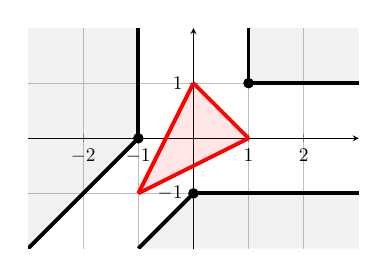
\begin{tikzpicture}[scale=0.7][line cap=round,line join=round,x=1cm,y=1cm]
 \begin{axis}[
 x=1cm,y=1cm,
 axis lines=middle,
 ymajorgrids=true,
 xmajorgrids=true,
 xmin=-3,
 xmax=3,
 ymin=-2,
 ymax=2,
 xtick={-2,...,2},
 ytick={-1,0,1}
 ]
 \fill[line width=2pt,color=red,fill=red,fill opacity=0.1] (0,1) -- (1,0) -- (-1,-1) -- cycle;
 
 \fill[line width=2pt,fill=gray,fill opacity=0.1] (-1,0) -- (-1,2) -- (-3,2) -- (-3,-2) -- cycle;
 \fill[line width=2pt,fill=gray,fill opacity=0.1] (1,1) -- (1,2) -- (3,2) -- (3,1) -- cycle;
 \fill[line width=2pt,fill=gray,fill opacity=0.1] (0,-1) -- (-1,-2) -- (3,-2) -- (3,-1) -- cycle;
 
 \draw [line width=2pt,color=red] (0,1)-- (1,0);
 \draw [line width=2pt,color=red] (1,0)-- (-1,-1);
 \draw [line width=2pt,color=red] (-1,-1)-- (0,1);
 
 \draw [line width=2pt] (-1,0)-- (-1,2);
 \draw [line width=2pt] (-3,-2)-- (-1,0);
 \draw [line width=2pt] (1,1)-- (1,2);
 \draw [line width=2pt] (3,1)-- (1,1);
 \draw [line width=2pt] (0,-1)-- (-1,-2);
 \draw [line width=2pt] (3,-1)-- (0,-1);
 \begin{scriptsize}
 \draw [fill=black] (1,1) circle (2.5pt);
 \draw [fill=black] (0,-1) circle (2.5pt);
 \draw [fill=black] (-1,0) circle (2.5pt);
 \end{scriptsize}
 \end{axis}
\end{tikzpicture}

\end{document}